\section{Curve Sketching}\label{sec:sketch}


We have been learning how we can understand the behaviour of a function based on its first and second derivatives. While we have been treating the properties of a function separately (increasing and decreasing, concave up and concave down, etc.), we combine them here to produce an accurate graph of the function without plotting lots of extraneous points.

Why bother? Graphing utilities are very accessible, whether on a computer, a hand--held calculator, or a smartphone. These resources are usually very fast and accurate. We will see that our method is not particularly fast -- it will require time (but it is not \textit{hard}). So again: why bother?

We are attempting to understand the behaviour of a function $f$ based on the information given by its derivatives. While all of a function's derivatives relay information about it, it turns out that ``most'' of the behaviour we care about is explained by \fp\ and \fpp. Understanding the interactions between the graph of $f$ and \fp\ and \fpp\ is important. To gain this understanding, one might argue that all that is needed is to look at lots of graphs. This is true to a point, but is somewhat similar to stating that one understands how an engine works after looking only at pictures. It is true that the basic ideas will be conveyed, but ``hands--on'' access increases understanding.

The following Key Idea summarizes what we have learned so far that is applicable to sketching graphs of functions and gives a framework for putting that information together. It is followed by several examples.

\enlargethispage{2\baselineskip}
%\setboxwidth{200pt}
%\hskip-200pt
%\begin{minipage}{\textwidth+200pt}
%\small
\keyidea{idea:sketch}{Curve Sketching}
{To produce an accurate sketch a given function $f$, consider the following steps.\index{curve sketching}
\begin{enumerate}
\item		Find the domain of $f$. Generally, we assume that the domain is the entire real line then find restrictions, such as where a denominator is 0 or where negatives appear under the radical.
\item 		Find the $x$- and $y$-intercepts of $f$, if possible; construct a sign diagram for $f$.
\item		Find the location of any vertical asymptotes of $f$ (usually done in conjunction with item 2 above). Use your sign diagram to determine whether $f(x)$ is approaching $\infty$ or $\-infty$ on either side of each vertical asymptote.
\item		Consider the limits $\ds\lim_{x\to-\infty}f(x)$ and $\ds\lim_{x\to\infty}f(x)$ to determine the end behaviour of the function.
\item		Compute  $\fp$, and find the critical points of $f$.
%\item		Create a number line that includes all critical points, possible points of inflection, and locations of vertical asymptotes. For each interval created, determine whether $f$ is increasing or decreasing, concave up or down.
%\item		Evaluate $f$ at each critical point and possible point of inflection. Plot these points on a set of axes. Connect these points with curves exhibiting the proper concavity. Sketch asymptotes and $x$ and $y$ intercepts where applicable.
\end{enumerate}
\small\textit{(continued)}\normalsize
}
\addtocounter{keyideacounter}{-1}
\keyidea{idea:sketchb}{Curve Sketching -- Continued}
{%To produce an accurate sketch a given function $f$, consider the following steps.
\begin{enumerate}\addtocounter{enumi}{5}
%\item		Find the domain of $f$. Generally, we assume that the domain is the entire real line then find restrictions, such as where a denominator is 0 or where negatives appear under the radical.
%\item		Find the critical values of $f$.
%\item		Find the possible points of inflection of $f$.
%\item		Find the location of any vertical asymptotes of $f$ (usually done in conjunction with item 1 above).
%\item		Consider the limits $\lim_{x\to-\infty}f(x)$ and $\lim_{x\to\infty}f(x)$ to determine the end behaviour of the function.
\item 		Construct a sign diagram for $\fp$; classify the critical points using the first derivative test. Determine the intervals on which $f$ is increasing or decreasing.
\item		Compute $\fpp$ and find the possible points of inflection of $f$. 
\item		Construct a sign diagram for $\fpp$, and determine the intervals on which the graph of $f$ is concave up or concave down.
\item 		Plot the intercepts and asymptotes of $f$ on a set of coordinate axes. Roughly sketch the behaviour of $f$ near the asymptotes.
Then plot the critical points and inflection points.
\item		Sketch the graph of $f$ by connecting the points plotted so far with curves exhibiting the proper concavity. Sketch asymptotes and $x$ and $y$ intercepts where applicable.
\end{enumerate}
}
%\restoreboxwidth
%\end{minipage}

\example{ex_sketch1}{Curve sketching}{
Use Key Idea \ref{idea:sketch} to sketch $f(x) = 3x^3-10x^2+7x+5$.}
{We follow the steps outlined in the Key Idea.
\begin{enumerate}
\item		The domain of $f$ is the entire real line; there are no values $x$ for which $f(x)$ is not defined.
\item		The $y$-intercept is given by $f(0)=5$. Determining the $x$-intercepts would involve finding the (quite likely irrational) zeros of a cubic polynomial, so we skip this step for now. (We may have to settle for approximate zeros later.) Since we don't know the zeros of $f$, we can't construct a sign diagram for $f$.
\item		There are no vertical asymptotes, since the domain of $f$ is $\mathbb{R}$.
\item		We determine the end behaviour using limits as $x$ approaches $\pm$infinity.				
\[
\lim_{x\to -\infty} f(x) = -\infty \qquad \lim_{x\to \infty}f(x) = \infty.
\]
			We do not have any horizontal asymptotes. (But it is still useful to know the direction in which the graph is headed at either end.)

\item		Find the critical points of $f$. We compute $\fp(x) = 9x^2-20x+7$. Use the Quadratic Formula to find the roots of $\fp$:
\[
x = \frac{20\pm \sqrt{(-20)^2-4(9)(7)}}{2(9)} = \frac19\left(10\pm\sqrt{37}\right) \Rightarrow x\approx 0.435, 1.787.
\]
\item 		Construct a sign diagram for $fp$. We found that the critical points of $f$ are 
\[
c_1 = \frac{10-\sqrt{37}}{9} < \frac{10+\sqrt{37}}{9} = c_2.
\]
With $fp(x) = 9(x-c_1)(x-c_2)$ we quickly see that $fp(x)>0$ for $x<c_1$ or $x>c_2$, and $fp(x)<0$ for $c_1<x<c_2$.

\pagebreak

The sign diagram for $fp$ is given by:

\noindent\begin{minipage}{\textwidth}
\begin{center}
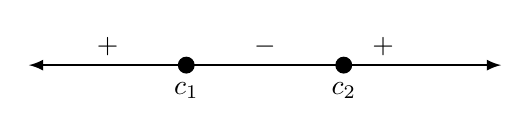
\begin{tikzpicture}[>=latex]
  \draw [thick, <->] (-2,0) -- (4,0);
  \draw [fill] (0.0,0) circle [radius =.1];
  \draw [fill] (2,0) circle [radius =.1];
  \node at (-1,0) [above] {$+$};
  \node at (1,0) [above] {$-$};
  \node at (2.5,0) [above] {$+$};
  \node at (0,-0.1) [below] {$c_1$};
  \node at (2,-0.1) [below] {$c_2$};
  \end{tikzpicture}
\end{center}
\captionsetup{type=figure}%
			\caption{Sign diagram for $\fp$ in Example \ref{ex_sketch1}.}\label{fig:sketchline1fp}
\end{minipage}

From the sign diagram, we see that $f$ is increasing on $(-\infty,c_1)\cup (c_2,\infty)$ (where $fp(x)>0$, and $f$ is decreasing on $(c_1,c_2)$ (where $fp(x)<0$).

Since $fp$ changes from positive to negative at $c_1$, we know that $(c_1,f(c_1))$ is a local maximum, and since $fp$ changes from negative to positive at $c_2$, we know that $(c_2,f(c_2))$ is a local minimum.

\item		Find the possible points of inflection of $f$. We compute $\fpp(x) = 18x-20$. We have 
\[
\fpp(x) = 0 \Rightarrow x= 10/9 \approx 1.111.
\]
\item		Construct a sign diagram for $\fpp$.
We have only one zero for $\fpp$, and we easily see that $\fpp(x)>0$ for $x>10/9$, and $\fpp(x)<0$ for $x<10/9$. The sign diagram for $\fpp$ is given below, with the critical points also indicated for reference:

\noindent\begin{minipage}{\textwidth}
\begin{center}
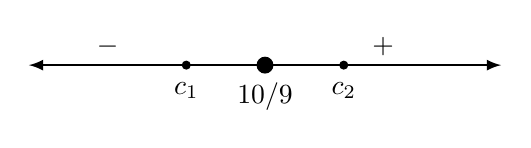
\begin{tikzpicture}[>=latex]
  \draw [thick, <->] (-2,0) -- (4,0);
  \draw [fill] (0.0,0) circle [radius =.05];
  \draw [fill] (2,0) circle [radius =.05];
  \draw [fill] (1,0) circle [radius =.1];
  \node at (-1,0) [above] {$-$};
  \node at (2.5,0) [above] {$+$};
  \node at (0,-0.1) [below] {$c_1$};
  \node at (2,-0.1) [below] {$c_2$};
  \node at (1,-0.1) [below] {$10/9$};
  \end{tikzpicture}
\end{center}
\captionsetup{type=figure}%
			\caption{Sign diagram for $\fpp$ in Example \ref{ex_sketch1}.}\label{fig:sketchline1fpp}
\end{minipage}


\item		We plot the appropriate points on axes as shown in Figure \ref{fig:sketch1}(a) and connect the points with straight lines. In Figure \ref{fig:sketch1}(b) we adjust these lines to demonstrate the proper concavity. Our curve crosses the $y$ axis at $y=5$ and crosses the $x$ axis near $x=-0.424$. In Figure \ref{fig:sketch1}(c) we show a graph of $f$ drawn with a computer program, verifying the accuracy of our sketch.
\end{enumerate}

\mtable{.6}{Sketching $f$ in Example \ref{ex_sketch1}.}{fig:sketch1}
%\mfigure{.8}{Beginning to sketch $f$ in Example \ref{ex_sketch1}.}{fig:sketch1a}{figures/figsketch1a}
%\mfigure{.57}{Adding concavity to the  sketch $f$ in Example \ref{ex_sketch1}.}{fig:sketch1b}{figures/figsketch1b}
%\mfigure{.34}{A computer generated graph of $f$ in Example \ref{ex_sketch1}.}{fig:sketch1}{figures/figsketch1}
}
\vskip-\baselineskip}\\

\example{ex_sketch2}{Curve sketching}{
Sketch $\ds f(x) = \frac{x^2-x-2}{x^2-x-6}$.}
{We again follow the steps outlined in Key Idea \ref{idea:sketch}.

\begin{enumerate}
		\item	In determining the domain, we assume it is all real numbers and look for restrictions. We find that at $x=-2$ and $x=3$, $f(x)$ is not defined. So the domain of $f$ is $D = \{\text{real numbers } x\ | \ x\neq -2,3\}$.
		\item The numerator of $f$ factors as $(x-2)(x+1)$, so $f(x)=0$ for $x=-1$ and $x=2$; these are the $x$-intercepts of $f$. The $y$-intercept is given by $f(0) = 1/3$.
		
Our function has two zeros and two points at which it is undefined. Note that $f(x)$ changes sign at each of these points, so we need to indicate each of them in our sign diagram. We use hollow dots to indicate the points at which $f$ is undefined, giving us the following sign diagram:

\noindent\begin{minipage}{\textwidth}
\begin{center}
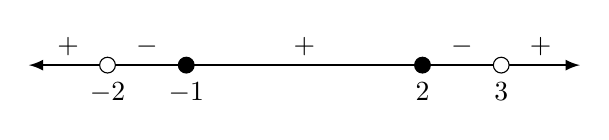
\begin{tikzpicture}[>=latex]
  \draw [thick, <->] (-3,0) -- (4,0);
  \draw [fill=white] (-2.0,0) circle [radius =.1];
  \draw [fill] (-1,0) circle [radius =.1];
  \draw [fill] (2,0) circle [radius =.1];
  \draw [fill=white] (3,0) circle [radius =.1];
  \node at (-2.5,0) [above] {$+$};
  \node at (-1.5,0) [above] {$-$};
  \node at (0.5, 0) [above] {$+$};
  \node at (2.5, 0) [above] {$-$};
  \node at (3.5, 0) [above] {$+$};
  \node at (-2,-0.1) [below] {$-2$};
  \node at (-1,-0.1) [below] {$-1$};
  \node at (2,-0.1) [below] {$2$};
  \node at (3,-0.1) [below] {$3$};
  \end{tikzpicture}
\end{center}
\captionsetup{type=figure}%
			\caption{Sign diagram for $f$ in Example \ref{ex_sketch2}.}\label{fig:sketchline2f}
\end{minipage}		

		\item We see from the sign diagram for $f$ in Figure \ref{fig:sketchline2f} that $f$ has vertical asymptotes at $x=-2$ and $x=3$; moreover, we can deduce the following asymptotic behaviour: at $x=-2$
\[
\lim_{x\to -2^-}f(x) = +\infty \quad \text{ and } \quad \lim_{x\to -2^+}f(x) = -\infty,
\]
and at $x=3$
\[
\lim_{x\to 3^-}f(x) = -\infty \quad \text{ and } \quad 
\lim_{x\to 3^+}f(x) = +\infty.
\]

		\item		There is a horizontal asymptote of $y=1$, as $\ds \lim_{x\to -\infty}f(x) = 1$ and $\ds\lim_{x\to\infty}f(x) =1$.

		\item		To find the critical values of $f$, we first find $\fp(x)$. Using the Quotient Rule, we find 
\[
\fp(x) = \frac{-8x+4}{(x^2+x-6)^2} = \frac{-8x+4}{(x-3)^2(x+2)^2}.
\]
		
		$\fp(x) = 0$ when $x = 1/2$, and $\fp$ is undefined when $x=-2,3$. Since \fp\ is undefined only when $f$ is, these are not critical values. The only critical value is $x=1/2$. The sign diagram for $\fp$ is given as follows:
		
\noindent\begin{minipage}{\textwidth}
\begin{center}
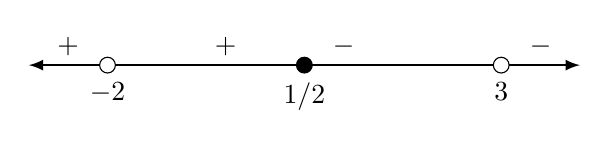
\begin{tikzpicture}[>=latex]
  \draw [thick, <->] (-3,0) -- (4,0);
  \draw [fill=white] (-2.0,0) circle [radius =.1];
  \draw [fill] (0.5,0) circle [radius =.1];
  \draw [fill=white] (3,0) circle [radius =.1];
  \node at (-2.5,0) [above] {$+$};
  \node at (-0.5,0) [above] {$+$};
  \node at (1, 0) [above] {$-$};
  \node at (3.5, 0) [above] {$-$};
  \node at (-2,-0.1) [below] {$-2$};
  \node at (0.5,-0.1) [below] {$1/2$};
  \node at (3,-0.1) [below] {$3$};
  \end{tikzpicture}
\end{center}
\captionsetup{type=figure}%
			\caption{Sign diagram for $\fp$ in Example \ref{ex_sketch2}.}\label{fig:sketchline2fp}
\end{minipage}		
	
	From the sign diagram for $\fp$, we see that $\fp(x)$ changes from positive to negative at $x=1/2$, so we have a local maximum at $(1/2,f(1/2))$. We also see that $f$ is increasing on $(-\infty,-2)\cup(-2,1/2)$ and decreasing on $(1/2,3)\cup (3,\infty)$.
		
		\item		To find the possible points of inflection, we find $\fpp(x)$, again employing the Quotient Rule: 
\[
\fpp(x) = \frac{24x^2-24x+56}{(x-3)^3(x+2)^3}.
\]
		
		\item We find that $\fpp(x)$ is never 0 (setting the numerator equal to 0 and solving for $x$, we find the only roots to this quadratic are imaginary) and \fpp\ is undefined when $x=-2,3$. Thus concavity will possibly only change at $x=-2$ and $x=3$. The sign diagram is given by:

\noindent\begin{minipage}{\textwidth}
\begin{center}
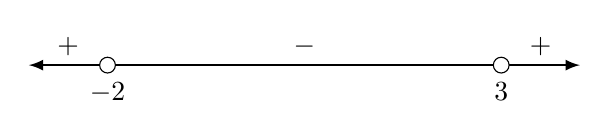
\begin{tikzpicture}[>=latex]
  \draw [thick, <->] (-3,0) -- (4,0);
  \draw [fill=white] (-2.0,0) circle [radius =.1];
  \draw [fill=white] (3,0) circle [radius =.1];
  \node at (-2.5,0) [above] {$+$};
  \node at (0.5, 0) [above] {$-$};
  \node at (3.5, 0) [above] {$+$};
  \node at (-2,-0.1) [below] {$-2$};
  \node at (3,-0.1) [below] {$3$};
  \end{tikzpicture}
\end{center}
\captionsetup{type=figure}%
			\caption{Sign diagram for $\fpp$ in Example \ref{ex_sketch2}.}\label{fig:sketchline2fpp}
\end{minipage}
		
From the sign diagram we see that the graph of $f$ is concave up on $(-\infty,-2)\cup (3,\infty)$ and concave down on $(-2,3)$		
		
	
		\item		In Figure \ref{fig:sketch2}(a), we plot the points from the number line on a set of axes and connect the points with straight lines to get a general idea of what the function looks like (these lines effectively only convey increasing/decreasing information). In Figure \ref{fig:sketch2}(b), we adjust the graph with the appropriate concavity. We also show $f$ crossing the $x$ axis at $x=-1$ and $x=2$.
\end{enumerate}
Figure \ref{fig:sketch2}(c) shows a computer generated graph of $f$, which verifies the accuracy of our sketch.

\enlargethispage{2\baselineskip}

\mtable{.4}{Sketching $f$ in Example \ref{ex_sketch2}.}{fig:sketch2}{%
\begin{tabular}{c}
\myincludegraphics{figures/figsketch2a}\\[10pt]
(a)\\[10pt]
\myincludegraphics{figures/figsketch2b}\\[10pt]
(b)\\[10pt]
\myincludegraphics{figures/figsketch2}\\[10pt]
(c)
\end{tabular}
%\mfigure{.8}{Beginning to sketch $f$ in Example \ref{ex_sketch2}.}{fig:sketch2a}{figures/figsketch2a}
%\mfigure{.57}{Adding concavity to the  sketch $f$ in Example \ref{ex_sketch2}.}{fig:sketch2b}{figures/figsketch2b}
%\mfigure{.34}{A computer generated graph of $f$ in Example \ref{ex_sketch2}.}{fig:sketch2}{figures/figsketch2}
}% ends if/then/else
\vskip-\baselineskip}\pagebreak

\example{ex_sketch3}{Curve sketching}{
Sketch $\ds f(x) = \frac{5(x-2)(x+1)}{x^2+2x+4}.$}
{We again follow Key Idea \ref{idea:sketch}.
	\begin{enumerate}
	\item		We assume that the domain of $f$ is all real numbers and consider restrictions. The only restrictions come when the denominator is 0, but this never occurs. Therefore the domain of $f$ is all real numbers, $\mathbb{R}$.
\item The $x$-intercepts of $f$ are $(-1,0)$, and $(2,0)$, and the $y$-intercept is $(0,-5/2)$. The sign diagram of $f$ is given below:

\noindent\begin{minipage}{\textwidth}
\begin{center}
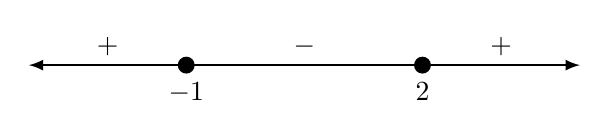
\begin{tikzpicture}[>=latex]
  \draw [thick, <->] (-3,0) -- (4,0);
  \draw [fill] (-1,0) circle [radius =.1];
  \draw [fill] (2,0) circle [radius =.1];
  \node at (-2,0) [above] {$+$};
  \node at (0.5, 0) [above] {$-$};
  \node at (3, 0) [above] {$+$};
  \node at (-1,-0.1) [below] {$-1$};
  \node at (2,-0.1) [below] {$2$};
  \end{tikzpicture}
\end{center}
\captionsetup{type=figure}%
			\caption{Sign diagram for $f$ in Example \ref{ex_sketch3}.}\label{fig:sketchline3f}
\end{minipage}	

    \item Since the domain of $f$ is $\mathbb{R}$, there are no vertical asymptotes.
    
    \item		We have a horizontal asymptote of $y=5$, as $\ds \lim_{x\to-\infty}f(x) = \lim_{x\to\infty}f(x) = 5$.
    
	\item		We find the critical values of $f$ by setting $\fp(x)=0$ and solving for $x$. We find 
\[
\fp(x) = \frac{15x(x+4)}{(x^2+2x+4)^2} \quad \Rightarrow \quad \fp(x) = 0 \text{ when } \ x=-4,0.
\]

	\item The sign diagram for $\fp$ is given by:
	
\noindent\begin{minipage}{\textwidth}
\begin{center}
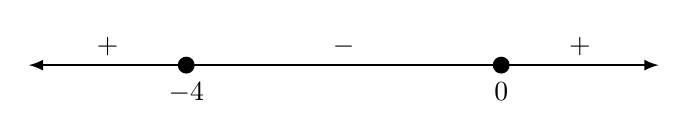
\begin{tikzpicture}[>=latex]
  \draw [thick, <->] (-6,0) -- (2,0);
  \draw [fill] (-4,0) circle [radius =.1];
  \draw [fill] (0,0) circle [radius =.1];
  \node at (-5,0) [above] {$+$};
  \node at (-2, 0) [above] {$-$};
  \node at (1, 0) [above] {$+$};
  \node at (-4,-0.1) [below] {$-4$};
  \node at (0,-0.1) [below] {$0$};
  \end{tikzpicture}
\end{center}
\captionsetup{type=figure}%
			\caption{Sign diagram for $\fp$ in Example \ref{ex_sketch3}.}\label{fig:sketchline3fp}
\end{minipage}	

From the sign diagram, we see that $\fp(x)$ changes from positive to negative at $x=-4$, so $(-4,f(-4))$ is a relative maximum, and $\fp(x)$ changes from negative to positive at $x=0$, so $(0,f(0))$ is a relative minimum. We also see that $f$ is increasing on $(-\infty,-4)\cup (0,\infty)$, and decreasing on $(-4,0)$.
	
	\item		We find the possible points of inflection by solving $\fpp(x) = 0$ for $x$. We find
\[
\fpp(x) = -\frac{30x^3+180x^2-240}{(x^2+2x+4)^3} .
\]
 The cubic in the numerator does not factor very ``nicely.'' We instead approximate the roots (with the help of a computer) at $c_1= -5.759$, $c_2=-1.305$ and $c_3=1.064$. The sign diagram for $\fpp$ is given by:
 
\noindent\begin{minipage}{\textwidth}
\begin{center}
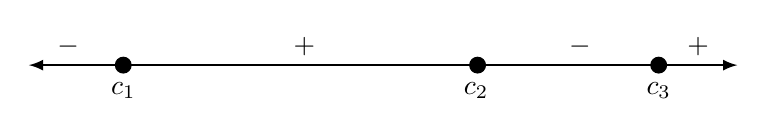
\begin{tikzpicture}[>=latex]
  \draw [thick, <->] (-7,0) -- (2,0);
  \draw [fill] (-5.8,0) circle [radius =.1];
  \draw [fill] (-1.3,0) circle [radius =.1];
  \draw [fill] (1,0) circle [radius =.1];
  \node at (-6.5,0) [above] {$-$};
  \node at (-3.5, 0) [above] {$+$};
  \node at (0, 0) [above] {$-$};
  \node at (1.5, 0) [above] {$+$};
  \node at (-5.8,-0.1) [below] {$c_1$};
  \node at (-1.32,-0.1) [below] {$c_2$};
  \node at (1,-0.1) [below] {$c_3$};
  \end{tikzpicture}
\end{center}
\captionsetup{type=figure}%
			\caption{Sign diagram for $\fpp$ in Example \ref{ex_sketch3}.}\label{fig:sketchline3fpp}
\end{minipage}	

\enlargethispage{\baselineskip}
	
	\item		In Figure \ref{fig:sketch3}(a) we plot the significant points from the number line as well as the two roots of $f$, $x=-1$ and $x=2$, and connect the points with straight lines to get a general impression about the graph. In Figure \ref{fig:sketch3}(b), we add concavity. Figure \ref{fig:sketch3}(c) shows a computer generated graph of $f$, affirming our results.		
	\end{enumerate}
	
\mtable{.5}{Sketching $f$ in Example \ref{ex_sketch3}.}{fig:sketch3}{%
\begin{tabular}{c}
\myincludegraphics{figures/figsketch3a}\\[10pt]
(a)\\[10pt]
\myincludegraphics{figures/figsketch3b}\\[10pt]
(b)\\[10pt]
\myincludegraphics{figures/figsketch3}\\[10pt]
(c)
\end{tabular}
%\mfigure{.8}{Beginning to sketch $f$ in Example \ref{ex_sketch3}.}{fig:sketch3a}{figures/figsketch3a}
%\mfigure{.57}{Adding concavity to the  sketch $f$ in Example \ref{ex_sketch3}.}{fig:sketch3b}{figures/figsketch3b}
%\mfigure{.34}{A computer generated graph of $f$ in Example \ref{ex_sketch3}.}{fig:sketch3}{figures/figsketch3}
}% ends if/then/else
\vskip-\baselineskip}\pagebreak

In each of our examples, we found a few, significant points on the graph of $f$ that corresponded to changes in increasing/decreasing or concavity. We connected these points with straight lines, then adjusted for concavity, and finished by showing a very accurate, computer generated graph. 

Why are computer graphics so good? It is not because computers are ``smart\-er'' than we are. Rather, it is largely because computers are much faster at computing than we are. In general, computers graph functions much like most students do when first learning to draw graphs: they plot equally spaced points, then connect the dots using lines. By using lots of points, the connecting lines are short and the graph looks smooth. 

This does a fine job of graphing in most cases (in fact, this is the method used for many graphs in this text). However, in regions where the graph is very ``curvy,'' this can generate noticeable sharp edges on the graph unless a large number of points are used. High quality computer algebra systems, such as \textit{Mathematica}, use special algorithms to plot lots of points only where the graph is ``curvy.''

In Figure \ref{fig:mathematica_sinx}, a graph of $y=\sin x$ is given, generated by \textit{Mathematica}. The small points represent each of the places \textit{Mathematica} sampled the function. Notice how at the ``bends'' of $\sin x$, lots of points are used; where $\sin x$ is relatively straight, fewer points are used. (Many points are also used at the endpoints to ensure the ``end behaviour'' is accurate.) 

\vskip\baselineskip
\noindent%
\begin{minipage}{\textwidth}\centering
\includegraphics{figures/figmathematica_sinx}
\captionsetup{type=figure}%
			\caption{A graph of $y=\sin x$ generated by \textit{Mathematica}.}\label{fig:mathematica_sinx}
\end{minipage}
\vskip\baselineskip

How does \textit{Mathematica} know where the graph is ``curvy''? Calculus. When we study \textit{curvature} in a later chapter, we will see how the first and second derivatives of a function work together to provide a measurement of ``curviness.'' \textit{Mathematica} employs algorithms to determine regions of ``high curvature'' and plots extra points there.

Again, the goal of this section is not ``How to graph a function when there is no computer to help.'' Rather, the goal is ``Understand that the shape of the graph of a function is largely determined by understanding the behaviour of the function at a few key places.'' In Example \ref{ex_sketch3}, we were able to accurately sketch a complicated graph using only 5 points and knowledge of asymptotes!

There are many applications of our understanding of derivatives beyond curve sketching. The next chapter explores some of these applications, demonstrating just a few kinds of problems that can be solved with a basic knowledge of differentiation. 

\printexercises{exercises/03_05_exercises}